\documentclass[12pt]{report}
\title{\textbf{\Huge View Maintenance \\ \large{in} \\ \Huge Data Warehousing } }
\author{CV Hariharan \bullet 1610110147 \\ Divya Raj \bullet 1610110123 \\ Devansh Purohit \bullet 1610110116}
\date{}

\usepackage[margin=1.4in]{geometry}
\usepackage{graphicx}
\usepackage{enumitem}
\usepackage{xcolor}
\usepackage{float}
\usepackage{amsmath}

\begin{document}
\maketitle
\section*{Acknowledgment}
We would like to thank Dr. Sonia Khetarpaul, our instructor for the Advance Database Management course this semester, for helping us with this project and the report. She taught us the concepts needed for this project and was available to us for help, whenever we needed it. Thank you.\\
\\We would also like to thank Hemant Jain and Anjana Gosain for their amazing paper titled "A Comprehensive Study of View Maintenance Approaches in 
Data Warehousing Evolution". It was a source of great help throughout this project. \\
\\Also, huge gratitude towards Abdulaziz S. Almazyad and Mohammad Khubeb Siddiqui for their paper titled "Incremental View Maintenance: An Algorithmic 
Approach". It gave us great insight into the incremental approach to view maintenance and inspired the final solution that we implemented.
\\\\Finally, we would like to thank Github user AntonioL for his repository -  "factorized-incremental-maintenance". It provided us a code wise basis for the project and helped us get started.
\\\\All the relevant links can be found at the end of this report in the Bibliography section.
\tableofcontents
\newpage
\renewcommand{\thesection}{\arabic{section}}
\section{Introduction}
A data warehouse mainly stores integrated information over data from 
many different remote data sources for query and analysis. The 
integrated information at the data warehouse is stored in the form of 
materialized views. Using these materialized views, user queries may be 
answered quickly and efficiently as the information may be directly 
available. These materialized views must be maintained in answer to 
actual relation updates in the different remote sources. \\
One of the issues 
related to materialized views is that whether they should be recomputed 
or they should be adapted incrementally after every change in the base 
relations. \\
View maintenance is the process of updating a materialized 
view in response to changes to the underlying data is called view 
maintenance. There are several algorithms developed by different 
authors to ease the problem of view maintenance for data warehouse 
systems. \cite{basic} \\
In this report, we document the already existing approaches in the field, describe the approach that we took and also show our findings and conclusions. 
\\\\First, some definitions-

\begin{description}[font=$\bullet$~\normalfont\scshape\color{orange!50!black}]
\item [Source] - A  database,  application,  file,  or  other  storage  facility  from which  the  data  in  a  data  warehouse  is  derived.  The  source contains  the  operating  data,  flat  files  and  stage  files.  The  
stage  file  receives  the  data  from  source  process  and  it  
verifies  its  credit-ability  and  the  required  data  files  will  be  
passed   to   warehouse   through   view   manager.   Source   
division also termed as top tier of architecture. \cite{saudi}
\item[Warehouse] - A relational database that is designed for query and analysis rather   than   transaction   processing.   A   data   warehouse
usually   contains   historical   data   that   is   derived   from transaction data, but it can include data from other sources. It  separates  analysis  workload  from  transaction  workload  and  enables  a  business  to  consolidate  data  from  several
sources.  It  contains  the  Summary  data,  raw  data,  metadata,
mined  data  etc.  Warehouse  division  also  termed  as  middle
tier of architecture. \cite{saudi}
\item[User] - Users   may   be   end   users   and   make   use   of   the   data warehouse   view   maintenance   in   the   Analysis   of   Data   
mining, Data reporting etc, and User division also termed as 
top tier of the architecture. \cite{saudi}
\end{description}

\section{Existing and Related Work}
Various  approaches  have  been  introduced  for  maintaining  
the view in a warehouse environment. 
\begin{figure}[H]
\centering 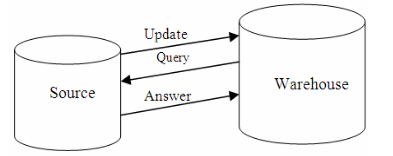
\includegraphics[width=0.7\textwidth]{images/pic1.png}
\caption{Basic Approach}
\end{figure}
\begin{description}[font=$\bullet$~\normalfont\scshape\color{blue!50!black}]
\item[Basic Algorithm] In Fig 1, it is shown that there 
is communication between Source and  the  warehouse,  when  update  occurs  at  source,  it  sends the  notification  to  warehouse  later  on  warehouse  sends  the query  to  source  for  the  corresponding  update  as  source  
receives the query it sends the answer to warehouse to that corresponding query.\\
\\1. When  an  update  occurs at  the  source,  it  sends  the update notification to the warehouse. 
\\2. Warehouse  receives  the  notification  and  sends  
back the query to the source about the update. 
\\3. Source receives the query    sent    by    the    
warehouse and returns the answer to that query.  
\\\\The   basic   algorithm   is   neither   convergent   nor   weakly   
consistent in warehouse environment. \cite{saudi}
\item[Recompute View] RV does not rely on incremental view maintenance 
approach. It is based on recomputation of materialized view 
from the scratch. When ever the update occurs at the source 
it recomputes the view from the scratch. In RV approach 
warehouse sends the Query to the source asking it to 
recompute the view from the scratch after certain number of 
updates. RV sends 2 messages for each update. The bytes 
transferred are much higher
 in RV than the relative 
algorithms. \\This degrades the performance of RV \cite{saudi}
\\\item[Eager Compensating Algorithm]
COLLECT =  
\\W $up_i$
: receive $U_i$; 
\begin{center}
Let $Q_i$
= v($U_i$) – 
$_{Q}\in_{UQS}Q_j(U_i) $
\\send $Q_i$ to the source; 
\\trigger event S $qu_i$ at the source 
\end{center}
W $ans_i$: receive $A_i$; 
\begin{center}
        let COLLECT = COLLECT + $A_i$; 
\\        if UQS =
           \\then { MV ←MV + COLLECT; COLLECT ←} 
\\        else do nothing. 
\end{center}
ECA is an incremental view maintenance algorithm. It is a 
method   for   fixing   the   view   maintenance   problem   that   
occurs  due  to  the  decoupling  between  base  data  and  the  
view maintenance manager at the warehouse. The key idea 
of  the  ECA  algorithm  is  that  it  cannot  rely  on  the  state  of  
the     base     information     that     is     continuously     being     
updated/modified  by  the  sources.  It  must  keep  track  of  the  
updates  received  from  the  source  and  then  filter  out  i.e.,  
compensate any information that will duplicate the resulting 
queries. By subtracting (or adding) the results it knows that 
will (not) get in future queries, it will create an accurate end 
result for the view.
\\The above algorithm states that: 
Initially  the  COLLECT  will  be  empty,  source  executes  an  
update  ($U_i$)  and  the  notification  sent  to  the  warehouse.  
Warehouse  receives  the  source  update ($U_i$)  and  sends  the  
query ($Q_i$)     based on  ($U_i$), for each query in     
UQS(Unanswered Query Set: the set of query set that were 
sent by the warehouse, but answers have not been received)
formulates  a  compensating  Query $Q_j$ based on $U_i$ and $Q_i$ with $Q_j$. Warehouse receive the query result and update the 
Materialized  View(MV),  the  result  of  the  query  should  be  
applied to the Materialized View(MV) only after the answer 
to this query and all related compensating query have been 
received. 
To   avoid   invalid   state   ECA   collects   the   intermediate   
answers  in  relation  denote
d  as  COLLECT  (initially  its  
empty).\cite{saudi}
\item[Lazy Approach] Lazy approach maintains the view in a lazy manner that 
relieves the updates of the maintenance overhead as in the 
incremental view maintenance approaches. View 
maintenance is postponed unt
il the system has free cycles 
or it is referenced by any query. These free cycles are utilized for the view maintenance that relieves the updates 
and queries from the overhead
. The updates are combined 
from different transactions into a single maintenance task. It 
also exploits row versioning. In lazy maintenance the 
updates do not maintain the view it just stores the required 
information so that the affect
ed views can be maintained 
later. It actually uses system free cycles to maintain the 
views, in this no updates or queries pay for the maintenance 
task. But, in case the view is not
 up to date and query is sent 
over it, then the particular query has to pay for all part of 
the view maintenance and some
delay also. However, it 
pays only the view maintenance that it uses and not for 
other views \cite{basic}
\end{description}

\section{Proposed Approach}
We made an approach which is a hybrid of the incremental and the recompute view approach. \\Consider a base relation P(a, b, c) with a materialized view V(A, B), where V.A maps to P.a and V.B maps to P.b .
\begin{figure}[H]
\centering 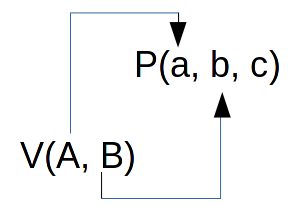
\includegraphics[width=0.4\textwidth]{images/mapping.png}
\caption{Mapping between base table and the view}
\end{figure}
\begin{enumerate}
  \item When the view V is made, 3 triggers are made on P, for insert, update and delete, which will be used later to update the views.
  \item Upon inputting the query, the query is first parsed to get the corresponding views, base tables and the operations to be performed.
  \item Meanwhile, a query is made to get the mapping between the source's and the warehouse's column. For example, in the case of P and V, to figure out that V.A = P.a
  \item If the query on the base table is simple (i.e does not contain joins, only selection and projections) go to 6, else go to 5.
  \item Simple query - \textbf{Incremental approach}, i.e send a command to the view to recompute itself, i.e delete the previous existence, and recalculate the base table query that forms it. Save it to disk. End.
  \item Complex query - \textbf{Recompute View}, i.e send a query to the view which updates the view instead of recalculating it. This happens by the insert, update and delete triggers that were defined earlier on the base table. End.\\
\end{enumerate}
\begin{figure}[H]
\centering 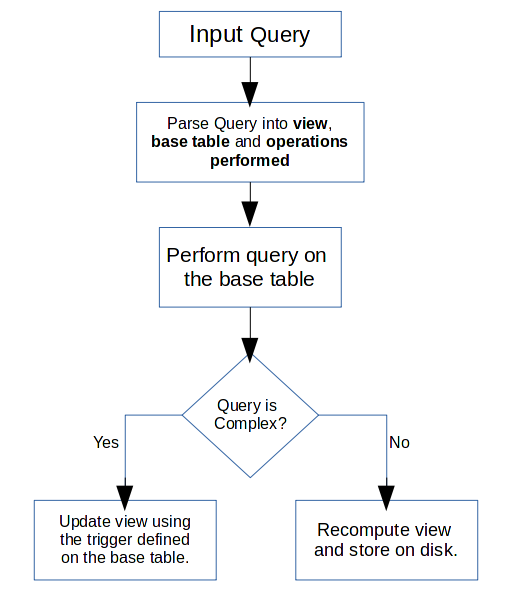
\includegraphics[width=0.8\textwidth]{images/flowchart.png}
\caption{Basic flowchart of the implementation}
\end{figure}

\section{Implementation and Results}
To implement our algorithm, we worked with Google Big Query, which is Google's serverless, highly scalable, enterprise data warehouse designed to make our data analysis on a warehouse without worrying about the logistics of it all. \cite{gcp} 
\\\\ We wrote our code in the python programming language and used the 'bigquery', 'sqlparse' and 'mysql' libraries to assist us.
\\\\We used the openly available StackOverflow dataset as our dummy data warehouse. The dataset is of size 57 GB and has 4 tables and 3 view, as shown in Figure 4.
\begin{figure}[H]
\centering 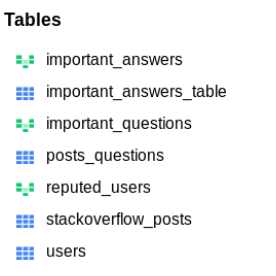
\includegraphics[width=0.4\textwidth]{images/so.png}
\caption{Tables and View in the Dataset (Blue = table, Green = view)}
\end{figure}
\begin{enumerate}
	\item Connect to the GCP client using the API key provided, so that we can work with the StackOverflow Dataset.
	\item Input a query. Parse it to find out the view, base table(s) and the SQL command involved.
	\item If a new view is to be formed from a base table, say 'important\_answers\_table', set up triggers for the base table- 
		\begin{enumerate}
			\item Insert- Set up an insert trigger which sends an appropriate query to the view when an insertion of a new answer takes place on the base table.
			\item Update- An update trigger which sends an update query to the view when values are updated in the base table.
			\item Delete- A delete trigger which deletes the corresponding answer from the view as it was deleted in the base table.
		\end{enumerate}
	\item Figure out the mappings from view to base table. An example result output of step 3 and 4 is shown in Figure 5.
		\begin{figure}[H]
		\centering 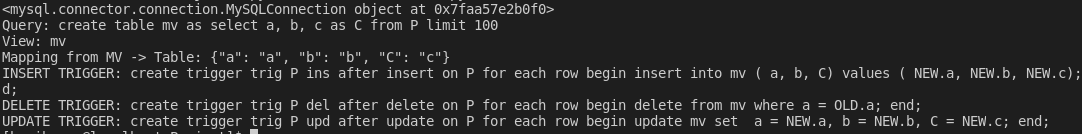
\includegraphics[width=1\textwidth]{images/mvq.png}
		\caption{View mapping and trigger formation output}
		\end{figure}
	\item Execute the query on the base table, save the result.
	\item Based on if the query has more than one tables mentioned after 'from' in the statement. it's classified as simple(1 table) or complex(>1 table). If a query is 					simple go to step 7 else execute step 8 and then go to step 9.
	\item Query is simple, hence the corresponding trigger executes and the value is either inserted, updated or deleted in the view, changes are saved to disk.
	\item Query is complex, hence the existing view is deleted and a new view is recalculated. This new view is then saved.
	\item End.
\end{enumerate}
\pagebreak
\section{Limitations and Conclusions}
The approach that we've taken is really basic and has a few limitations.
\\The obvious one is the recomputation of the view the query made is complex i.e contains joins etc. That is one thing we would want to improve in the future. This can be done by having a logging system between the view and the base table, which can be used to calculate the diffs instead of the entire view again.
Another limitation is that our solution is not as scalable as some of the existing approaches (notably ECA). It runs smoothly on our StackOverflow dataset, but will mostly struggle in terms of performance when used on bigger and more varied datasets.
\\\\In conclusion, we would like to say that even though we were not able to implement some of the advanced view maintenance algorithms, this project gave us an opportunity to study about these algorithms thoroughly, and develop a theoretical understanding about them.
\\The actual implementation that we did, gave us good insight into how materialized views are maintained practically. This gave us an opportunity to extend what we had learned in the class and build something practical that could reinforce our learning of the concept.
\begin{thebibliography}{999}
\bibitem{saudi}
Abdulaziz S. Almazyad and Mohammad Khubeb Siddiqui\emph{ Incremental View Maintenance: An Algorithmic 
Approach}.
 	 Feb, 2016.
\bibitem{basic}
Hemant Jain Anjana Gosain \emph{A Comprehensive Study of View Maintenance Approaches in Data Warehousing Evolution }.
 	 Sept, 2012. 	 
\bibitem{gcp}
Google Big Query Documentation \emph{https://console.cloud.google.com/bigquery/docs}.
\bibitem{git}
AntonioL \emph{github.com/AntonioL/factorized-incremental-maintenance}
\end{thebibliography}
\end{document}